\documentclass[../main.tex]{subfiles}

\begin{document}

\section{MQTT topics}

We can see the used MQTT topics in \textbf{Figure \ref{fig:mqtt-topics}}, defined specifically in \textbf{Section \ref{sec:player-topics}, \ref{sec:state-topics}}.

\subsection{Player topics}
\label{sec:player-topics}

With the base topic \textbf{players/<player\_id>/}, where \textit{player\_id} is the player's predefined unique identifier (e.g. in our case \textit{duo\_jc}), we have the following separated topics, where the \textit{actions} subtopics are used to send feedback from the players and the \textit{state} subtopics are used to receive feedback from the game controller:

Player actions topics:
\begin{itemize}
    \item \textbf{actions/die}: \textit{bool}. Indicates the player's death.
    \item \textbf{actions/move}: \textit{bool}. Indicates the player's movement.
    \item \textbf{actions/shoot}: \textit{bool}. Indicates the player's shooting decision.
    \item \textbf{actions/ready/meeple}: \textit{bool}. Indicates the player's meeple is ready.
    \item \textbf{actions/ready/base}: \textit{bool}. Indicates the player's base is ready.
\end{itemize}

Player state topics:
\begin{itemize}
    \item \textbf{state/has\_bullet}: \textit{bool}. Indicates if the player has the bullet.
    \item \textbf{state/has\_won}: \textit{bool}. Indicates if the player is the last alive.
    \item \textbf{state/has\_died}: \textit{bool}. Indicates if the player has died.
    \item \textbf{state/can\_move}: \textit{bool}. Indicates if it's the player's turn to move.
\end{itemize}

\subsection{State topics}
\label{sec:state-topics}

With the base topic \textbf{state/}, we have the following topics:

\begin{itemize}
    \item \textbf{stage}: \textit{"joining" | "moving" | "shooting" | "end"}. Indicates the current game stage for all the players.
\end{itemize}

\begin{figure}
    \centering
    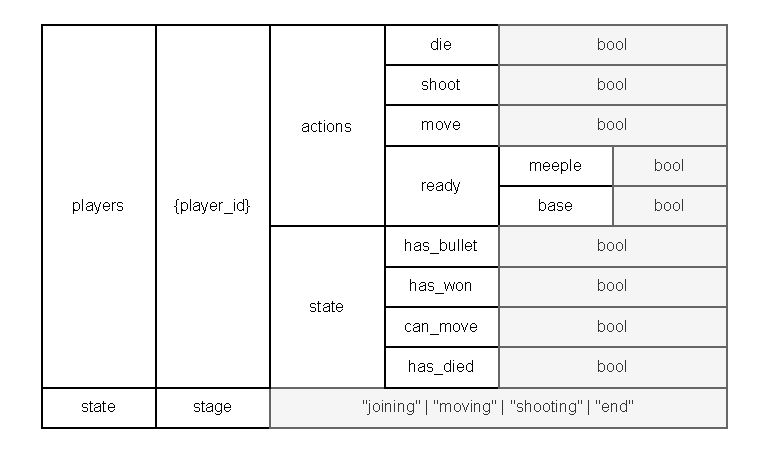
\includegraphics[width= 0.8\linewidth]{../media/figures/mqtt-topics.pdf}
    \caption{MQTT topics resume}
    \label{fig:mqtt-topics}
\end{figure}


\end{document}

